\chapter{ML deep dive D: the choices we tested, and the ML question bank}
\label{ch:deepeval}

Every dial in the new model was chosen by an experiment, not a feeling. This part lists each experiment with its real numbers, then gives you an extra bank of ML-specific questions.

\section{The two alternatives that treat the workload explicitly}

\subsection{The control chart: the new model without the load factor}
\begin{simplebox}
The simplest possible fix is to drop the learned shape entirely and judge each signal against its own recent median and spread, with the bursty-signal protection. That is the \emph{control chart} version of the model: the same code with the load factor switched off (\code{mode: 'control'}). It does not claim to know the shape of traffic, so it does not call a new traffic level ``unusual in shape''. It already gets the time in alarm to 0\% on both workload recordings. What it lacks is the ability to \emph{explain} a change: after a big shift, the first readings are still far from the old median, so a few false alarm episodes remain (1.2 and 1.9 per hour).
\end{simplebox}

\subsection{The subspace (PCA) model: the principled multivariate alternative}
\begin{simplebox}
The subspace model comes from network monitoring. Suppose you measure every signal of every service. The \emph{shared causes} (how busy the project is, the time of day) push many numbers up and down together. In a table of readings these shared movements span only one or two ``directions''. The model finds those directions from recent healthy data (principal components) and treats everything along them as explained. An anomaly is what sticks out \emph{off} those directions. It is elegant, and it works: 1\% and 3\% of time in alarm on the two workload recordings (one component), 50\% caught-and-named on the live faults, the best of any model on that set.

Why we did not adopt it: it raised 7.7 to 10.7 false-alarm episodes per hour on the steady load steps; it adapts more slowly to a new load pattern; and its cost grows faster than linearly because the covariance has one row per service-signal pair (1.2 seconds per window at 320 services against 0.12 s for the load factor).
\end{simplebox}

\begin{techbox}
\code{pcaModel.ts}: standardise every signal of every ready service by its slow reference (median) and tail-aware spread; load $=$ the median of the network-in/out shifts when at least four values exist; keep a window of healthy standardised vectors (keys \code{service|feature}); every 10 accepted vectors refit the covariance and extract the top 1--2 eigenvectors by power iteration with deflation; the residual of a new vector $e=u-UU^\top u$ (after centring) is scaled per coordinate by the residual's spread over the healthy window (floor $0.35$); one-sided features count only upward; the level is $\max z/4$. The same gate and drift rules apply.
\end{techbox}

\section{The sweeps, with real numbers}
For each sweep the other settings stay at their defaults. Columns: C+N (caught and named) and FA/h (false alarms per hour) on the real, live and synthetic sets, and the two workload recordings (FA/h and alarm time).

\subsection{The alarm line $z_{\text{line}}$ (the most important dial)}
\begin{center}
\scriptsize
\setlength{\tabcolsep}{3pt}
\begin{tabular}{rcccccc}
\toprule
$z_{\text{line}}$ & Real (C+N / FA) & Live (C+N / FA) & Synth. (C+N / FA) & Organic (FA / alarm) & Steps (FA / alarm)\\
\midrule
2 & 71 / 8.5 & 44 / 8.2 & 79 / 1.0 & 15.0 / 11\% & 16.5 / 11\%\\
3 & 71 / 3.8 & 45 / 8.2 & 83 / 1.4 & 5.8 / 2\% & 2.9 / 0\%\\
\textbf{4} & \textbf{71 / 2.3} & \textbf{48 / 0.0} & \textbf{78 / 0.2} & \textbf{0.0 / 0\%} & \textbf{1.0 / 0\%}\\
5 & 68 / 0.8 & 49 / 0.0 & 75 / 0.2 & 0.0 / 0\% & 1.0 / 0\%\\
6 & 66 / 0.8 & 49 / 0.0 & 73 / 0.0 & 0.0 / 0\% & 1.0 / 0\%\\
8 & 68 / 0.8 & 49 / 0.0 & 66 / 0.0 & 0.0 / 0\% & 1.0 / 0\%\\
\bottomrule
\end{tabular}
\end{center}
\begin{simplebox}
Think of the alarm line as a volume knob. Turn it low (2) and the model is jumpy: it catches every fault (real detection 94\%, synthetic 100\%) but fires on workload swings (15 false episodes per hour, 11\% of calm time in alarm). Turn it high (8) and it is silent but misses faults (synthetic detection falls to 75\%). The value 4 is the \emph{loosest} setting that keeps both workload recordings quiet, so it is the most sensitive quiet setting.
\end{simplebox}
\begin{figure}[H]
\centering
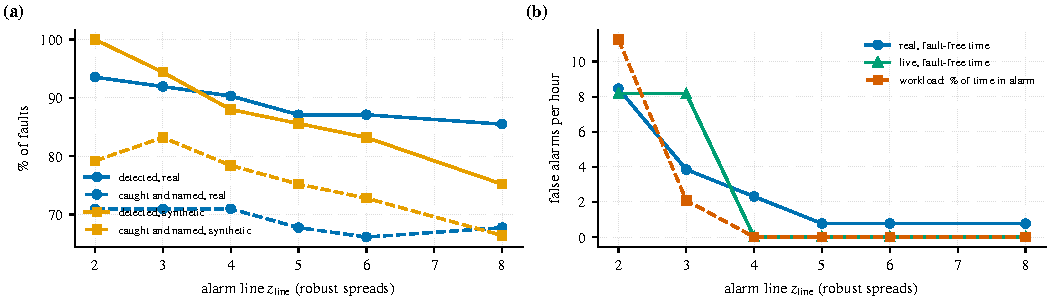
\includegraphics[width=0.98\textwidth]{fig_zline.pdf}
\caption{Sensitivity of the load-aware model to its alarm line (alarm at level 2, that is at twice the line).}
\end{figure}

\subsection{The training window}
\begin{center}
\small
\begin{tabular}{rcccc}
\toprule
Window & Real FA/h & Live FA/h & Organic (FA / alarm) & Steps (FA / alarm)\\
\midrule
60 & 1.5 & 8.2 & 10.4 / 9\% & 7.7 / 6\%\\
\textbf{120} & 2.3 & 0.0 & 0.0 / 0\% & 1.0 / 0\%\\
240 & 1.5 & 0.0 & 0.0 / 0\% & 1.9 / 0\%\\
\bottomrule
\end{tabular}
\end{center}
\begin{simplebox}
Too short a window (60 readings, five minutes) does not hold enough of the signal's natural wobble, so the spread is underestimated and the workload recordings become noisy again. 120 is enough; 240 does not help.
\end{simplebox}

\subsection{The slow reference length}
\begin{simplebox}
120, 360 and 720 readings (10, 30 and 60 minutes) all give essentially the same result (only 120 raised 1.2 false episodes per hour on the organic recording). It matters little once it is long enough; we kept 30 minutes.
\end{simplebox}

\subsection{The drift time for mild shifts}
\begin{center}
\small
\begin{tabular}{rcccc}
\toprule
Readings & Real FA/h & Real alarm time & Synth. detected & Synth. C+N\\
\midrule
\textbf{24 (2 min)} & 2.3 & 6\% & 88\% & 78\%\\
48 (4 min) & 3.1 & 13\% & 89\% & 78\%\\
72 (6 min) & 3.1 & 13\% & 90\% & 78\%\\
120 (10 min) & 3.1 & 13\% & 90\% & 78\%\\
240 (20 min) & 3.1 & 13\% & 90\% & 78\%\\
\bottomrule
\end{tabular}
\end{center}
\begin{simplebox}
We wanted to make the model alarm for longer on mild faults, so we tried longer drift times. It changed nothing on accuracy (caught-and-named stayed at 71\% real, 78\% synthetic) and nothing on the workload recordings, but \emph{doubled} the time in alarm on the real systems (6\% to 13\%) and raised false alarms from 2.3 to 3.1 per hour, because a service whose footprint changes after a restart stays in alarm until accepted. So we kept two minutes and documented the consequence.
\end{simplebox}

\subsection{The range guard (rejected)}
\begin{center}
\small
\begin{tabular}{rcc}
\toprule
Range guard $k$ floors beyond the window range & Steps FA/h & Steps alarm time\\
\midrule
\textbf{off (0)} & 1.0 & 0\%\\
4 & 4.8 & 1\%\\
6 & 2.9 & 0\%\\
10 & 1.0 & 0\%\\
\bottomrule
\end{tabular}
\end{center}
\begin{simplebox}
The old engine had a range guard (``a value far outside what you have seen counts as level 1''). We tried carrying it over to the new model. It changed no result on any fault set and \emph{added} false alarms on the steady-load steps (4.8 per hour at $k=4$ against 1.0 without it). So the new model has none: the robust spread, with its tail-aware part, already scales to the jump.
\end{simplebox}

\subsection{The spread: MAD against tail-aware}
\begin{center}
\small
\begin{tabular}{lcccc}
\toprule
 & Real FA/h & Live FA/h & Organic alarm & Steps alarm\\
\midrule
Load factor, MAD spread & 3.8 & 16.3 & 10\% & 6\%\\
\textbf{Load factor, tail spread} & 2.3 & 0.0 & 0\% & 0\%\\
Control chart, MAD spread & 10.0 & 24.5 & 13\% & 31\%\\
Control chart, tail spread & 2.3 & 0.0 & 0\% & 0\%\\
\bottomrule
\end{tabular}
\end{center}
\begin{simplebox}
The tail-aware spread is the second-biggest improvement after dropping the forest. With the MAD alone, bursty signals look far more extreme than they are, and even the load factor alarms 10\% and 6\% of calm time. With the tail spread both are 0\%.
\end{simplebox}

\section{The ablation of the final model, explained}
\begin{center}
\small
\begin{tabular}{lcccc}
\toprule
 & \multicolumn{2}{c}{Real} & \multicolumn{2}{c}{Synthetic held-out}\\
Variant & C+N & Alarm time & C+N & Alarm time\\
\midrule
Full model & 71 & 6\% & 75 & 4\%\\
$-$ \code{docker stop} fact & 53 & 6\% & 60 & 4\%\\
$-$ crash-loop fact & 71 & 6\% & 68 & 4\%\\
$-$ load factor & 71 & 6\% & 75 & 4\%\\
$-$ tail-aware spread & 71 & 12\% & 75 & 5\%\\
$-$ random walk & 68 & 6\% & 73 & 4\%\\
$-$ one-sided features & 69 & 24\% & 75 & 0\%\\
$-$ two-speed drift & 71 & 13\% & 74 & 14\%\\
Alarm at level 1 instead of 2 & 73 & 12\% & 77 & 7\%\\
\bottomrule
\end{tabular}
\end{center}
\begin{simplebox}
Read the table by columns. \textbf{C+N column:} only the \code{docker stop} fact (53 against 71) and the crash-loop fact (68 against 75 on synthetic) change how many faults are caught and named, plus the walk by a few points. \textbf{Alarm-time column:} the statistical mechanisms (tail spread, one-sided features, two-speed drift) are what keep the model quiet: without one-sided features alarm time on the real systems goes from 6\% to 24\%. The load factor does not change either column on \emph{injected} faults, because the load does not move in them; its value shows only on the workload recordings (Part~\ref{ch:mlstory}).
\end{simplebox}

\begin{saybox}
``Different mechanisms earn their keep on different measures: the facts decide how many faults we catch and name, and the statistical machinery decides whether we stay quiet. The load factor is invisible on injected faults and decisive on workload changes, and that is exactly why we also measured workload changes.''
\end{saybox}

\section{ML question bank}
Extra questions that go deeper than Part~\ref{ch:qa}.

\q{Walk me through what happens to one reading, from raw numbers to an alarm.}\\
\textbf{Answer:} Eight raw numbers are log-transformed (with units) into a vector. The load model compares each signal with the service's slow reference, takes the median shift over busy services as $L$, estimates slopes by ridge, and judges each signal against the service's accepted-window baseline after subtracting $bL$, under two hypotheses, keeping the smaller deviation. The max over signals divided by 4 is the level. If the level holds two readings, it becomes an anomaly (0 below level 0.5, 1 at level 2) and enters the random walk; facts count as level 10. The Hybrid alarms if a fact holds, or the largest level reaches 2, or the rule score reaches 1.25 times its line.

\q{Why log-transform?}\\
\textbf{Answer:} Workload changes are multiplicative, so on a log scale ``twice as busy'' is the same step for a service at 10 requests and one at 10\,000, which lets one load factor describe all services. The unit inside the log stops tiny flows on idle services from turning into big jumps.

\q{Why is the load factor a median and not a regression across services?}\\
\textbf{Answer:} A median is robust: a fault that distorts one or two services cannot move it, so it measures the shared change even while a fault is present. A regression would be pulled by the faulty service.

\q{What if only one service carries traffic?}\\
\textbf{Answer:} Then the load factor is not computed (it needs at least two contributing services) and stays 0. The model then behaves like the control chart.

\q{What if the whole project is faulty, for example the host runs out of memory?}\\
\textbf{Answer:} Then ``everyone moved together'' can look like load. But memory and throttling have slope prior 0, so they are not explained by load; the model only subtracts load from signals that follow it. Container facts (restarts, OOM exits) also raise the alarm directly.

\q{Why two hypotheses instead of just using the learned slope?}\\
\textbf{Answer:} The slope is estimated for a signal across the project; an individual service might ignore the load (a message bus) or follow it (a gateway). Trying both and keeping the smaller deviation handles both before either has been seen to move, and with the load unchanged both agree.

\q{Doesn't taking the minimum over hypotheses hide real faults?}\\
\textbf{Answer:} It can, if a fault happens to look like a load-following move. The risk is largest for a fault that begins during a very large load change. That is stated in the limitations, and the facts and the rules (which do not use the load factor) are a second line.

\q{How does the model avoid learning a fault?}\\
\textbf{Answer:} Only readings under level 1 join the window. A mild shift becomes normal after 24 readings, a large one after 360. So a mild fault is absorbed after two minutes; the rules and facts keep alarming.

\q{Why not just retrain the forest more often?}\\
\textbf{Answer:} A forest of the readings can never explain a workload change, however fresh it is: after a change it would still be in alarm until the window refills, then the window contains the new workload. The problem is not staleness; it is that the model has no notion of load.

\q{Is a deeper neural model a better fix?}\\
\textbf{Answer:} It could learn load dependence if given enough labelled variety, but that needs training data and is not auditable. Our fix is one extra estimate (the median shift) and a subtraction.

\q{How do you know the load factor works rather than just the tail spread?}\\
\textbf{Answer:} Two comparisons. With the tail spread, the control chart already has 0\% time in alarm but still 1.2 and 1.9 false episodes per hour on the two workload recordings; adding the load factor gives 0.0 and 1.0. With the MAD spread, the control chart is in alarm 31\% of the stepped-load recording and the version with the load factor 6\%, so the load factor removes most of the load-driven alarms even when the spread is poor. The tail spread is the larger part of the improvement; the load factor removes what remains.

\q{What is the ridge for, if the slope came out at the prior anyway?}\\
\textbf{Answer:} In our toy case and in much of the data, the load varies little and the prior (slope 1) is right. The ridge prevents wild slopes when the load has barely varied, and lets the slope adapt when it has.

\q{Why is memory not load-following?}\\
\textbf{Answer:} Memory in these services is dominated by fixed footprints, caches and leaks, not by instantaneous traffic; a prior slope of 0 means memory growth is never explained away by load, which is right for leaks.

\q{Why are errors and latency judged only upward?}\\
\textbf{Answer:} Lower error or latency than usual is never a fault of the service, and it follows every restart. Counting it would raise false alarms.

\q{Why do you ignore errors and latency below five requests?}\\
\textbf{Answer:} An error share computed from fewer than five requests is meaningless (one failure out of two is 50\%). So those two signals are treated as missing in that interval.

\q{Why is the first judgement delayed to 30 readings?}\\
\textbf{Answer:} A baseline and a spread need data. Below 30 readings (two and a half minutes) the median and MAD are too uncertain. Until then the service is \emph{not ready} and only container facts apply.

\q{What does ``accepted'' mean on a reading?}\\
\textbf{Answer:} That it was allowed into the training window: it was normal (level under 1), or it was a mild deviation that has lasted 24 readings, or a large one that has lasted 360.

\q{How is the old model's cost spike explained?}\\
\textbf{Answer:} Each service retrains its forests every ten accepted readings. With many services their schedules coincide, so the cost shows 95th-percentile windows nine times the mean. The new model refreshes baselines every four readings, with a peak about three times the mean.

\q{If the load-aware model is not more accurate, why replace the forest?}\\
\textbf{Answer:} Because accuracy on injected faults was never the defect. The defect was a false alarm on every service at every workload change, which the forest cannot fix and the load model does. We also cut the cost by 2.5 times at 320 services.

\q{Why not use the subspace model, which has the best live C+N?}\\
\textbf{Answer:} It is as good at discriminating but raised 7.7--10.7 false episodes per hour on steady load steps, adapts slowly, and costs more as services grow. The load factor was quieter and cheaper. If a project had few services and a strongly shared load, the subspace model would be a reasonable alternative.

\q{Did you test the ML on a system it had never seen?}\\
\textbf{Answer:} On 16 random synthetic topologies scored once, yes. On real systems, we only have our two benches, and the settings were not tuned on a held-out real system; we say the real numbers are optimistic by an unmeasured margin.

\q{What is the single weakest assumption of the load model?}\\
\textbf{Answer:} That the shared workload is a single scalar that all busy services follow with a common slope. If different services follow different parts of the traffic (for example batch jobs and user traffic), a single factor is too crude. The two-hypothesis test softens this, and a multi-factor model is future work.
